% This is samplepaper.tex, a sample chapter demonstrating the
% LLNCS macro package for Springer Computer Science proceedings;
% Version 2.21 of 2022/01/12
%
\documentclass[runningheads]{llncs}
%

\usepackage[T1]{fontenc}
% T1 fonts will be used to generate the final print and online PDFs,
% so please use T1 fonts in your manuscript whenever possible.
% Other font encondings may result in incorrect characters.
\usepackage{amsmath}
\usepackage{graphicx}

% Used for displaying a sample figure. If possible, figure files should
% be included in EPS format.
%
% If you use the hyperref package, please uncomment the following two lines
% to display URLs in blue roman font according to Springer's eBook style:
\usepackage{color}
%\renewcommand\UrlFont{\color{blue}\rmfamily}
%

\begin{document}


\title{Data Augmentation for EEG Motor Imagery Classification using Diffusion Model}
%
%\titlerunning{Abbreviated paper title}
% If the paper title is too long for the running head, you can set
% an abbreviated paper title here
%
\author{Nutapol Soingern \and
Akraradet Sinsamersuk\and
Chaklam Silpasuwanchai  }
%
\authorrunning{Nutapol S.\and et al.}
% First names are abbreviated in the running head.
% If there are more than two authors, 'et al.' is used.
%
\institute{Asian Institute of Technology, School of Engineering and Technology, Data Science and Artificial Intelligence, Pathum Thani, Thailand \email{chaklam@ait.asia} 
}
%
\maketitle              % typeset the header of the contribution
%
\begin{abstract}
\begin{sloppypar}
  Motor imagery classification using electroencephalogram (EEG) signals is an important research topic that has been extensively studied in the field of brain-computer interfaces (BCIs). However, due to the limited amount of available data, possibility of overfitting is a challenge, especially when using a deep-learning classifier. One way to address this is by performing data augmentation. This paper investigates the efficacy of the diffusion model as a data augmentation method for motor imagery classification. We evaluated the diffusion method by comparing it with commonly-used EEG data augmentation techniques namely such as Noise Addition,
  Fourier Transform Surrogates, Frequency Shift, and SmoothTimeMask. The result shows that the diffusion method outperformed other methods in terms of classification accuracy by 17.49\%. The Kullback–Leibler (KL) divergence is used for assessing the similarity between the training set (with and without augmentation) and validation set, thus showing the effectiveness of the diffusion approach compared to other techniques.
\end{sloppypar}

\keywords{Motor Imagery  \and EEG \and Brain Computer Interface \and Deep Learning \and Data Augmentation \and Diffusion \and KL divergence.}
\end{abstract}
%
%
%
\section{Introduction}

Brain-computer interfaces (BCI) establish a direct pathway between the human brain and a computer via signal processing and decoding techniques.  One classic paradigm of EEG is motor imagery (MI), in which its physiological basis is based on body movements or imagined movements that can produce $\alpha$ (8–13 Hz) and $\beta$ (13–30 Hz) event-related synchronization (ERS) and event-related desynchronization (ERD) rhythms in the motor-sensory areas of the brain \cite{wolpaw2013brain}. Recently, deep learning (DL) model has been used for motor imagery classification. For example, EEGNet \cite{lawhern2018eegnet} is a compact convolutional neural network designed for EEG-based brain-computer interfaces that effectively extracts spatial-temporal features from EEG signals. In any case, the paucity of data is a prevalent issue in the field of EEG classification, as it hinders the development and performance of DL models.  Consequently, a common symptom is overfitting, which reduces the model's accuracy and robustness on test set \cite{bilbao2017overfitting}. 

Data augmentation (DA) has been widely used to improve the robustness and accuracy of DL by artificially increasing the number of training data.  Traditional EEG data augmentation methods include \texttt{Noise Addition} \cite{wang2018data,parvan2019transfer,li2019channel}, fourier transform surrogates \cite{schwabedal2018addressing}, \texttt{Frequency Shift}ing \cite{rommel2021cadda,rommel2022data} and \texttt{\texttt{SmoothTimeMask}} \cite{mohsenvand2020contrastive}. 
\texttt{Noise Addition} \cite{li2019channel,parvan2019transfer} adds random white noise to all channels.  Fourier transform surrogates \cite{schwabedal2018addressing} randomizes the Fourier-transform (FT) phases of temporal-spatial data and generates surrogates that approximate examples from the data-generating distribution. \texttt{Frequency Shift}ing \cite{rommel2021cadda,rommel2022data} randomly shifts the frequency spectrum on all channels. Last, \texttt{\texttt{SmoothTimeMask}} \cite{mohsenvand2020contrastive} randomly masks consecutive time steps of the EEG signal and replaces them with zeros, in which the motivation is to force the model to disregard minor irrelevant events.

Recently, diffusion model \cite{ho2020denoising} was proposed which generates synthetic data based on Langevin dynamics. These models naturally admitted a progressive lossy decompression scheme. 
Diffusion mode has been used as a DA method to generate synthetic training data for skin disease classification \cite{akrout2023diffusion}, prostate cancer detection \cite{hao2021comprehensive}, chest X-ray imaging \cite{motamed2021data}, etc.   
%\textcolor{red}{Here you need to clearly explain what is \texttt{WaveGrad} but in a very precise and succinct manner.  The below sentence is extremely vague.....}

%Moreover, \texttt{WaveGrad} has been demonstrated in prior work \cite{chen2020\texttt{WaveGrad}} on score matching \cite{song2020sliced} and diffusion models. This model was formerly utilized to synthetically generate high-fidelity audio. Thus, adapting the diffusion model for MI-EEG and utilizing the model for DA is possible.

%\textcolor{red}{argue why WaveGrad; also need to mention how you modify it.....also in method}
In this work,  we demonstrated the use of the diffusion model for the purpose of data augmentation.  Particularly, we developed our diffusion model based on \texttt{WaveGrad} \cite{chen2020wavegrad} as a DA method for motor imagery classification.  \texttt{WaveGrad} has been initially for the purpose of audio waveforms generation.  The proposed approach involves utilizing score matching \cite{song2020sliced} and diffusion probabilistic models to estimate gradients of the data density within a conditional model. \texttt{WaveGrad} are success on audio waveforms generation. As a result, we implement this technique in to EEG signal domain. We modify \texttt{WaveGrad} by adjust about sequence length.   It involves initializing the model with a Gaussian white noise signal and subsequently improving the signal quality through an iterative process that utilizes a gradient-based sampler that is conditioned on the mel-spectrogram. We evaluated the effect of the proposed method by performing DA on BCI Competition IV 2a \cite{brunner2008bci} with various size of synthetic data with five standards EEG MI models (EEGNet \cite{lawhern2018eegnet}, ATCNet \cite{altaheri2022physics}, EEG-ITNet \cite{salami2022eeg}, Deep ConvNet \cite{schirrmeister2017deep} and ShallowFBCSPNet \cite{schirrmeister2017deep}). The proposed method improve the performance outperform other traditional EEG data augmentation methods. 

\section{Related Work}

\begin{sloppypar}    
We reviewed commonly-used data augmentation for EEG MI such as \texttt{Noise Addition}, \texttt{Fourier Transform Surrogates}, \texttt{Frequency Shift} and \texttt{SmoothTimeMask}.
\end{sloppypar}

\subsection{Noise Addition}
\texttt{Noise Addition} has two main categories for adding noise to the EEG signals for the purpose of DA \cite{lashgari2020data}.  First category regards to adding various types of noise, such as Gaussian noise, Poisson noise, salt-and-pepper noise, etc., each of which has its own set of parameters (such as mean and standard deviation), to the original signal.  The second category converts EEG signals to image sequences, then added noise to the resulting image sequences. In any case, the introduction of noise to the training data is assumed to enhance the robustness of the model by compelling it to learn features that were less susceptible to minor fluctuations in the data.  Indeed, such simulation of EEG data variability was commonly utilized to replicate the effects of electrode noise or subject movement during experimental procedures.  Previous research has demonstrated that the inclusion of Gaussian noise in EEG signals enhances the efficacy of the MI classification model when applied to BCI competition IV dataset 2b \cite{brunner2008bci} , resulting in a 10\% improvement in performance.


% A common technique in EEG research involved introducing Gaussian noise with zero mean and a standard deviation of 0.1 to the recorded data \cite{parvan2019transfer}.  

 %Specifically, Gaussian noise improve approximately 10\% in the classification accuracy compared to using no data augmentation\cite{parvan2019transfer}. %Overall, adding Gaussian noise is a simple yet effective way to increase the variability of EEG data, which can help improve the robustness and generalization performance of the motor imagery classification model.

\subsection{Fourier transform surrogates}
The Fourier transform surrogates (\texttt{FTSurrogate}) method utilizes the phase data of frequency elements, which were subsequently rearranged in a random manner while maintaining their original magnitude spectrum \cite{schwabedal2018addressing}. The generation of synthetic data samples has been utilized as a means to address the underrepresentation of certain classes. This approach has been shown to improve the balance of class distribution and enhance the accuracy of classification. The method proposed in this study has the potential to enhance classification performance either as a standalone technique or in conjunction with other data augmentation methods \cite{schwabedal2018addressing}. The extent of enhancement varies based on the particular dataset and classification issue. Terzano et al. \cite{terzano2001atlas} improved the mean F1-score by 7\% of a convolutional neural network utilized for sleep stage classification through the implementation of surrogate-based augmentation on the CAPSLPDB sleep database.
 %Fourier transform surrogates are a useful tool for addressing class imbalance in noisy signal classification problems, particularly when the underrepresented class has unique spectral characteristics that can be preserved through the surrogate generation process.

\subsection{Frequency Shift}

In the \texttt{Frequency Shift} method, the frequency spectrum of an EEG signal was randomly shifted to a different frequency range while maintaining the amplitude spectrum \cite{rommel2022data}. The proposed technique involved generating novel EEG signals that exhibit identical spectral characteristics as the initial signal, albeit with altered frequencies.  The \texttt{Frequency Shift} method was successful in enhancing the classification accuracy of certain EEG datasets. In the \texttt{Frequency Shift} method on motor imagery datasets, the implementation of the \texttt{Frequency Shift} method resulted in a 2.5\% increase in classification accuracy when compared to the baseline method. Moreover, this technique has been compared with various other transformation techniques to generate augmentated EEG signals \cite{rommel2021cadda}. The study assessed the efficacy of a novel method on various EEG classification tasks and demonstrated its superiority over conventional data augmentation techniques, including random cropping and flipping, as well as other learned data augmentation methods. The study's findings indicated that the suggested approach yields optimal performance and requires less time for training compared to gradient-based methods in the class-agnostic context. Additionally, it surpassed gradient-free methods in the class-wise context. The research paper lacked a specific numerical value for the quantity of effects or enhancements. The effectiveness of this method in enhancing classification performance was also observed in the BCI Competition IV 2a dataset \cite{brunner2008bci}.

\subsection{SmoothTimeMask}
\texttt{SmoothTimeMask} is a research methodology that utilizes time-domain augmentation to introduce smoothness into a signal. This is achieved by masking contiguous time intervals \cite{mohsenvand2020contrastive}.  This method involved generating a mask by randomly selecting a starting point and masking a fixed length of contiguous samples. A common technique used to create a smooth transition between masked and unmasked regions is the application of a convolution with a Gaussian kernel to the mask. The introduction of smoothness in the augmented signal has the potential to prevent overfitting and enhance the generalization of the model \cite{mohsenvand2020contrastive}  \textcolor{red}{need evidence of its effectiveness. The technique was used in other tasks of EEG. The result looks interesting so we include this technique in our work.}.

%EEG signal was performed with a filter in the band pass filter band of 8–35 Hz.

\subsection{WaveGrad}

\texttt{WaveGrad} is a generative model for waveform generation that uses score matching and denoising to improve the quality of generated waveforms. The basic idea behind the method is to estimate the probability density function of a dataset using a generative model, and then use this estimate to generate new data points that are similar to the original data.

To achieve this, \texttt{WaveGrad} uses an autoregressive architecture that predicts each sample of the waveform conditioned on the previous samples. Specifically, \texttt{WaveGrad} uses a modified version of the WaveNet architecture that replaces the dilated convolutions with a set of learned gates and skips connections, which reduces the computational cost of the model.

\texttt{WaveGrad} trains the generative model using score matching, which is a technique that involves matching the gradient of the log-density function of the model to the gradient of the true log-density function of the data. The idea behind score matching is that the gradient of the log-density function is easier to estimate than the function itself and that matching the gradients is sufficient to match the distributions.

Score matching is a technique used for estimating the probability density function (\texttt{PDF}) of a dataset by matching the score function of a model to the true score function of the \texttt{PDF}. The score function is the gradient of the log-density function, i.e., the vector of partial derivatives of the log-density function with respect to each input variable.

In score matching, the model is trained to minimize the difference between the score function of the model and the true score function of the \texttt{PDF}. This can be formulated as the following loss function:

\begin{equation}
L(\theta) = \sum_i |\nabla_x \log p(x_i; \theta) - \nabla_x \log \hat{p}(x_i)|^2
\end{equation}
where $\theta$ are the parameters of the model, $x_i$ is a data point, $p(x_i; \theta)$ is the model's probability density function, and $\hat{p}(x_i)$ is the true probability density function of the dataset.

Denoising score matching is an extension of score matching that uses a denoising autoencoder to estimate the score function of the \texttt{PDF}. The denoising autoencoder is trained to remove noise from the input data, and the score function of the denoised data is used to estimate the true score function of the \texttt{PDF}. The loss function for denoising score matching is:

\begin{equation}
L(\theta) = \sum_i |\nabla_x \log \hat{p}(\tilde{x}_i) - \nabla_x \log \hat{p}(x_i)|^2
\end{equation}

where $\tilde{x}_i$ is the denoised version of $x_i$.

Weighted denoising score matching is a further extension of denoising score matching that accounts for noisy labels. The idea is to assign higher weights to samples with less noise and lower weights to samples with more noise. This can be achieved by introducing a weighting function $w(x_i)$ into the loss function:

\begin{equation}
L(\theta) = \sum_i w(x_i) |\nabla_x \log \hat{p}(\tilde{x}_i) - \nabla_x \log \hat{p}(x_i)|^2
\end{equation}

where $\theta$ are the parameters of the model, $x_i$ is a data point, $\hat{p}(x_i)$ is the true probability density function of the dataset, $\tilde{x}_i$ is the denoised version of $x_i$, and $w(x_i)$ is a weighting function that assigns a weight to each sample based on the level of noise in its label.

In addition, \texttt{WaveGrad} further improves the optimization of the model by using a variant of stochastic gradient descent called Stochastic Gradient Hamiltonian Monte Carlo (SGHMC). SGHMC uses Hamiltonian dynamics to simulate the motion of particles in a potential energy landscape, which improves the exploration of the parameter space during optimization.

Overall, \texttt{WaveGrad} is able to generate high-quality waveforms that are comparable to or better than previous state-of-the-art methods. It achieves this by combining denoising and score matching with a modified version of the WaveNet architecture and SGHMC optimization. Although this technique shows its performance in the context of generating human voice audio \cite{chen2020wavegrad}, it should also work under an EEG signal because the sampling rate of the EEG signal is much lower than the audio domain.

\section{Methodology}
We compared the diffusion method against four DA methods and the baseline method without augmentation. Figure \ref{fig:System Diagram} shows how the training sets were obtained using different combinations of the DA method and sampling size.  The sampling size was chosen at the ratio of 25, 50, 75, 100\%.  Five commonly-used models for MI classification was used. The models were trained using subject-dependent scheme and evaluated on their respective testing sets. 

\begin{figure}[ht]
  \centering
  \caption[System Diagram]{\label{fig:System Diagram} Showed how to obtain training sets when using traditional DA and \texttt{WaveGrad}. \texttt{WaveGrad} was trained for each EEG channel in each class for each subject. Thus, we trained a total of 792 models from four classes, 22 channels and 9 subjects.}
  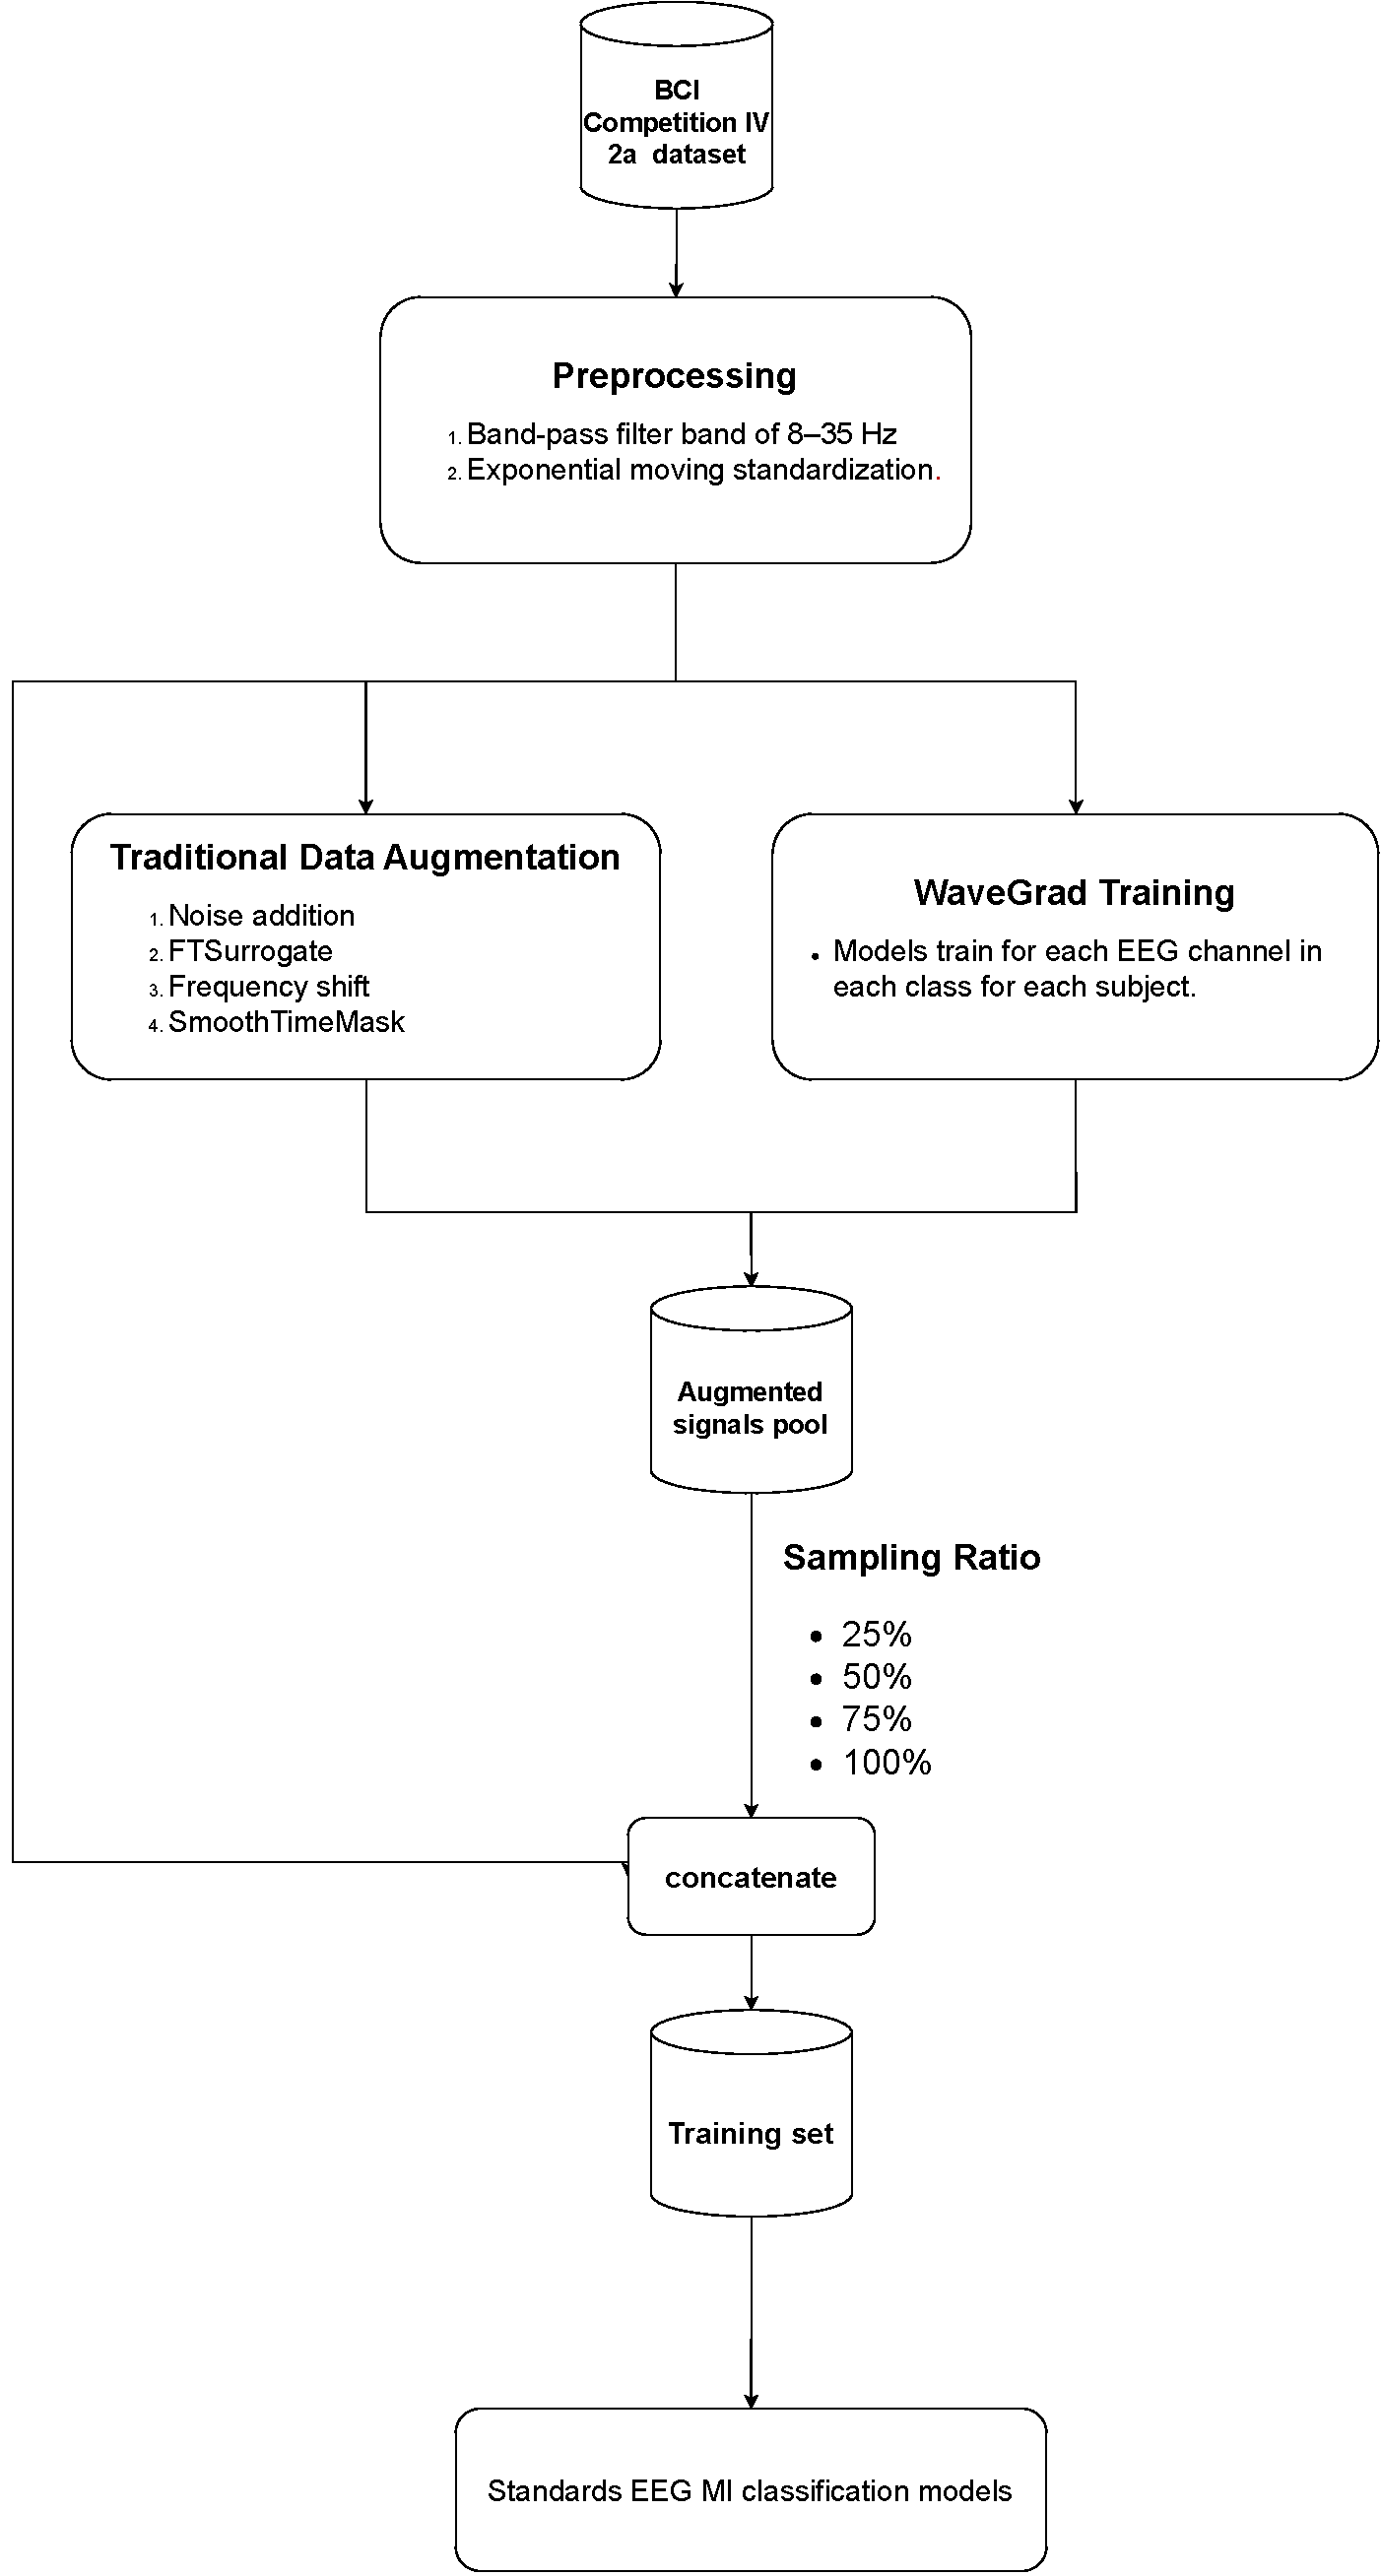
\includegraphics[width=0.6\textwidth]{fig/dyagram.pdf}
  \label{fig:System}
\end{figure}
%(b) Showed how to obtain training set when using \texttt{WaveGrad}.  \textcolor{red}{change to one diagram...}
\subsection{Datasets}

BCI Competition IV 2a \cite{brunner2008bci} was a collection of EEG data from 9 subjects who participated in a cue-based BCI paradigm involving four distinct motor imagery tasks: imagining movement of the left hand (class 1), the right hand (class 2), both feet (class 3) and the tongue (class 4). Each subject completed the tasks in two distinct sessions on different days, with each session consisting of six runs separated by brief pauses, resulting in a total of 48 trials (12 for each of the four classes). The data were captured while the participants sat in a comfortable armchair in front of a computer screen, and a fixation cross appeared at the start of each trial. A cue consisting of an arrow pointing to the left, right, down, or up was used to prompt the subjects to perform the desired motor imagery task. The subjects were instructed to perform the motor imagery task until the fixation cross disappeared from the screen without receiving any feedback. Signals were sampled at 250 Hz and filtered between 0.5 Hz and 100 Hz using a 50 Hz notch filter in order to reduce line noise. We used one section for training sets and another for test sets.

\subsection{Data Preprocessing}
EEG signal was filtered with a band pass filter of 8 - 35 Hz followed by exponential moving standardization $x_{\rm t}$. For exponential moving standardization, we computed the exponential moving mean $m_{\rm t}$ at time $t$ as shown in equations (\ref{eq1}).
Then, we computed the exponential moving variance $v_{\rm t}$ at time $t$ as shown in equation (\ref{eq2}).
we set $\texttt{factornew}$ as 0.001 and $\texttt{esp}$ as 0.0001. Finally, we standardized the data point $x_{\rm t}$ at time $t$ as shown in equation (\ref{eq3}).

\begin{eqnarray} 
m_{\rm t} = \text{factornew} \cdot \text{mean}(x_{\rm t}) + (1 - \text{factornew}) \cdot m_{\rm t-1}, \label{eq1}\\
v_{\rm t} = \text{factornew}\cdot (m_{\rm t} - x_{\rm t})^{2} + (1 - \text{factornew}) \cdot v_{\rm t-1} , \label{eq2} \\ 
x_{\rm t}^{'}  = \frac{(x_{\rm t}-m_{\rm t})}{\text{max}(\sqrt{->v_{\rm t}},\text{esp}), \label{eq3} }
\end{eqnarray}

\subsection{Data Augmentation}
Our objective was to assess the performance of each DA method with different ratios of augmented/synthetic data. Five DA methods (\texttt{Noise Addition}, \texttt{FTSurrogate}, \texttt{Frequency Shift}, \texttt{SmoothTimeMask}, \texttt{WaveGrad}) and four ratios (25\%, 50\%, 75\%, 100\%) = 20 combinations (5 methods x 4 ratios) of the training set are to be created.  Here, ratios refer to the amount of augmented/synthetic data used.  For example, given 25\% ratio, a 25\% augmented data is randomly sampled and add to the original training set.  By comparing different ratios, we can better understand the impact of number of augmentation to accuracy improvement.

\begin{sloppypar}
Similar to previous works \cite{rommel2021cadda,mohsenvand2020contrastive,leeb2008bci,terzano2001atlas}, we used the subject-dependent scheme which augments data in subject level (i.e., each subject is treated separately) and channel level (i.e., each channel is treated independently).
\end{sloppypar}
%The process of \texttt{Noise Addition} 

\textcolor{red}{add paper source for each technique}

\subsubsection{Noise Addition}: \texttt{Noise Addition} entails the inclusion of diverse forms of noise, such as Gaussian, Poisson, and others, that possess varying parameters to the original EEG signal. The raw EEG signal was subjected to additive noise by incorporating a Gaussian distribution with a standard deviation of 0.1. 

\subsubsection{Fourier Transform Surrogates}:
\texttt{Fourier transform surrogates} are a type of data generated by randomizing the phases of temporal-spatial data.


\subsubsection{Frequency Shift}: The technique of \texttt{Frequency Shift} is characterized by the alteration of the frequency of the EEG signal by a specific amount.
We random shift the frequency by \textpm2 Hz.

\subsubsection{SmoothTimeMask}:
\texttt{SmoothTimeMask} involves applying a smooth window function to mask a continuous segment of the signal, and optimizing it using gradient-based methods. The signal was randomly masked with a range of 100 sample points.

\subsubsection{WaveGrad}:
It is first important that \texttt{WaveGrad} is originally a generative model, not a formal augmentation technique.  Thus, in contrary to other DA methods, \texttt{WaveGrad} has to be trained before it can be used to generate a synthetic EEG signal.   The dataset consists of 9 subjects and four MI classes. The EEG recording has 22 channels. Thus, the total number of \texttt{WaveGrad} models was (9 subjects x 22 channels x 4 classes) = 792 models.  The training procedure and parameters were the same across all \texttt{WaveGrad} models. The learning rate was set to 0.0001 and the diffusion steps to 1000.  \textcolor{red}{talk more about what you add/modify}

\subsection{Evaluation}
First, we quantify the similarity between the set of raw EEG signals and the set of augmented/synthesized EEG signals using Kullback-Leibler divergence(KL divergence). This helps to explain why the augmentation works. By performing augmentation, we increase the variation of the training set such that the new variation overlaps with the testing set. Hence, the similarity between these two sets is higher. On the other hand, the similarity between the two sets is not changed or decreased if the new augmented signal creates a random noise instead of a new variation.

Second, once the quality of the augmented/synthetic data is quantified, we are now ready to quantify the usefulness of data augmentation techniques on actual EEG tasks.  We first selected five commonly-used motor imagery classification models (EEGNet, ATCNet, EEG-ITNet, Deep ConvNet and ShallowFBCSPNet) which would allow us to understand whether how complexity of the model relates with data augmentation.  Here, note that we simply define the complexity based on the model's number of parameters. Accuracy was then measured across all 21 combinations (5 DA methods x 4 sampling ratios + 1 baseline method without augmentation).  The details of each model were as follows:

\subsubsection{EEGNet}
%\textcolor{red}{intuition and parameters}
EEGNet is a single CNN architecture that can accurately classify EEG signals from different BCI paradigms while being as compact as possible. The authors introduced the use of depthwise and separable convolutions to construct an EEG-specific model that encapsulates well-known EEG feature extraction concepts for BCI. They compared EEGNet to current state-of-the-art approaches across four BCI paradigms and showed that EEGNet generalizes across paradigms and achieved comparably high performance when only limited training data is available across all tested paradigms.

\subsubsection{ATCNet}
%\textcolor{red}{intuition and parameters}
ATCNet was initially developed for predicting the onset of epileptic seizures using electroencephalogram (EEG) signals. The ATCNet consists of two blocks: an attention-based temporal convolutional (ATC) block and a transformer-based classification (TC) block. The ATC block is used to extract relevant features from the EEG signals, while the TC block is used to classify the extracted features into seizure and non-seizure classes. The proposed model was evaluated using the BCI Competition IV-2a (BCI-2a) dataset. The obtained accuracy ranged from 60.5\% to 89.5\%.


\subsubsection{EEG-ITNet}
EEG-ITNet uses inception modules and causal convolutions with dilation to extract rich spectral, spatial, and temporal information from multi-channel EEG signals with less complexity than other existing end-to-end architectures. The paper also provided a methodology for achieving intuitive visualisation structures such as topographic maps. The proposed EEG-ITNet model showed up to 5.9\% improvement in classification accuracy compared to its competitors in different scenarios.

\subsubsection{Deep ConvNet}
The deep ConvNet had four convolution-max-pooling blocks, with a special first block designed to handle EEG input, followed by three standard convolution-max-pooling blocks and a dense softmax classification layer. The authors found that recent advances in machine learning, including batch normalization and exponential linear units, together with a cropped training strategy, boosted the Deep ConvNets decoding performance, reaching at least as good performance as the widely used filter bank common spatial patterns (FBCSP) algorithm.

\subsubsection{ShallowFBCSPNet}
The shallow ConvNet are similar to the transformations of FBCSP. Concretely, the first two layers of the shallow ConvNet perform a temporal convolution and a spatial filter, as in the deep ConvNet. These steps are analogous to the bandpass and CSP spatial filter steps in FBCSP.

\section{Results}

\subsection{Kullback-Leibler divergence(KL divergence).}

To understand the quality of the generated data, we measured the similarity of signal by KL divergence process. We measure the KL divergence comparing of train set and test set, test set and train set with 25\% of data augmentation, test set and train set with 50\% of data augmentation, test set and train set with 75\% of data augmentation, test set and train set with 100\% of data augmentation, test set and data augmentation and train set and data augmentation. We randomize the augmentation data for this process 100 times and averaged the result.

Overall, \textcolor{red}{summarize the result a bit krub}

\textcolor{red}{table caption is too small krub}

\begin{table}[ht]
  \centering
  \caption[The result of KL divergence ]{The result of the study of KL divergence of raw EEG dataset and data augmentation from \texttt{WaveGrad}.
}
\scalebox{.35}{
\begin{tabular}{|l|l|l|l|l|l|l|l|}
\hline
\multicolumn{1}{|l|}{Subject} &
  test set vs train set &
  test set vs tran set with 25\% Augmetation &
  test set vs tran set with 50\% Augmetation &
  test set vs tran set with 75\% Augmetation &
  test set vs tran set with 100\% Augmetation &
  Test set vs Augmentation &
  Train set vs Augmentation \\ \hline
1                             & 2949.63 & 2757.15 & 2623.40 & 2525.57 & 2486.21 & 1988.35 & 1582.51 \\
2                             & 1641.60 & 1887.98 & 2009.06 & 2118.49 & 2222.43 & 2749.47 & 2970.01 \\
3                             & 2203.27 & 2298.26 & 2382.90 & 2416.10 & 2410.30 & 2671.86 & 2800.51 \\
4                             & 2559.50 & 2390.33 & 2291.63 & 2240.40 & 2176.35 & 1775.89 & 2193.34 \\
5                             & 2238.52 & 2215.49 & 2170.81 & 2146.55 & 2167.71 & 2045.00 & 1870.57 \\
6                             & 1935.63 & 1999.40 & 2061.10 & 2067.91 & 2103.15 & 2247.53 & 2069.20 \\
7                             & 2704.38 & 2564.74 & 2482.31 & 2424.12 & 2381.11 & 2024.06 & 1808.16 \\
8                             & 3245.50 & 2946.14 & 2752.42 & 2628.08 & 2497.71 & 1779.83 & 1398.65 \\
9                             & 2313.45 & 2290.44 & 2253.48 & 2231.11 & 2201.39 & 2145.52 & 2123.10 \\ \hline
\multicolumn{1}{|l|}{Average} & 2421.27 & 2372.21 & 2336.35 & 2310.92 & 2294.04 & 2158.61 & 2090.67 \\ \hline
\end{tabular} }
\end{table} 



\begin{table}[ht]
  \centering
  \caption[The result of KL divergence ]{The result of the study of KL divergence of raw EEG dataset and data augmentation from \texttt{Noise Addition}.
}
\scalebox{.35}{
\begin{tabular}{|l|l|l|l|l|l|l|l|}
\hline
\multicolumn{1}{|l|}{Subject} &
  test set vs train set &
  test set vs tran set with 25\% Augmetation &
  test set vs tran set with 50\% Augmetation &
  test set vs tran set with 75\% Augmetation &
  test set vs tran set with 100\% Augmetation &
  Test set vs Augmentation &
  Train set vs Augmentation \\ \hline
1       & 3096.06 & 3098.35 & 3129.45 & 3084.07 & 3082.39 & 3136.14 & 5.50 \\
2       & 1825.54 & 1847.41 & 1842.47 & 1840.31 & 1847.95 & 1855.50 & 8.51 \\
3       & 1931.80 & 1902.96 & 1899.25 & 1896.77 & 1929.07 & 1883.10 & 0.79 \\
4       & 2236.07 & 2214.81 & 2234.90 & 2242.26 & 2226.55 & 2253.03 & 9.64 \\
5       & 2412.31 & 2428.51 & 2407.26 & 2424.61 & 2411.43 & 2417.18 & 2.90 \\
6       & 1658.42 & 1674.19 & 1682.36 & 1661.31 & 1654.97 & 1665.17 & 5.86 \\
7       & 2670.83 & 2656.17 & 2653.48 & 2647.57 & 2675.15 & 2627.48 & 3.02 \\
8       & 2492.82 & 2486.57 & 2499.74 & 2485.40 & 2502.85 & 2477.18 & 4.33 \\
9       & 2527.24 & 2556.71 & 2575.44 & 2532.34 & 2514.06 & 2534.68 & 3.69 \\ \hline
\multicolumn{1}{|l|}{Average} &  2316.79 & 2318.41 & 2324.93 & 2312.74 & 2316.05 & 2316.61 & 4.91 \\ \hline
\end{tabular} }
\end{table} 

\begin{table}[ht]
  \centering
  \caption[The result of KL divergence ]{The result of the study of KL divergence of raw EEG dataset and data augmentation from \texttt{FTSurrogate}.
}
\scalebox{.35}{
\begin{tabular}{|l|l|l|l|l|l|l|l|}
\hline
\multicolumn{1}{|l|}{Subject} &
  test set vs train set &
  test set vs tran set with 25\% Augmetation &
  test set vs tran set with 50\% Augmetation &
  test set vs tran set with 75\% Augmetation &
  test set vs tran set with 100\% Augmetation &
  Test set vs Augmentation &
  Train set vs Augmentation \\ \hline
1       & 3096.06 & 2923.06 & 2778.94 & 2705.45 & 2639.85 & 2161.28 & 1763.78 \\
2       & 1825.54 & 2057.60 & 2149.51 & 2285.96 & 2365.13 & 2890.44 & 2892.79 \\
3       & 1931.80 & 2037.76 & 2091.94 & 2106.68 & 2157.68 & 2393.08 & 2509.07 \\
4       & 2236.07 & 2209.30 & 2186.28 & 2157.86 & 2162.64 & 2087.45 & 1872.45 \\
5       & 2412.31 & 2348.90 & 2315.24 & 2255.40 & 2231.07 & 2062.80 & 1953.67 \\
6       & 1658.42 & 1811.03 & 1916.95 & 1992.26 & 2062.44 & 2411.42 & 2592.67 \\
7       & 2670.83 & 2545.19 & 2505.66 & 2502.45 & 2440.79 & 2195.68 & 1920.34 \\
8       & 2492.82 & 2421.70 & 2389.56 & 2381.83 & 2342.94 & 2220.79 & 2078.85 \\
9       & 2527.24 & 2448.97 & 2416.09 & 2369.63 & 2353.87 & 2208.62 & 2457.15 \\ \hline
\multicolumn{1}{|l|}{Average} & 2316.79 & 2311.50 & 2305.57 & 2306.39 & 2306.27 & 2292.40 & 2226.75 \\ \hline
\end{tabular} }
\end{table} 


\begin{table}[ht]
  \centering
  \caption[The result of KL divergence ]{The result of the study of KL divergence of raw EEG dataset and data augmentation from \texttt{SmoothTimeMask}.
}
\scalebox{.35}{
\begin{tabular}{|l|l|l|l|l|l|l|l|}
\hline
\multicolumn{1}{|l|}{Subject} &
  test set vs train set &
  test set vs tran set with 25\% Augmetation &
  test set vs tran set with 50\% Augmetation &
  test set vs tran set with 75\% Augmetation &
  test set vs tran set with 100\% Augmetation &
  Test set vs Augmentation &
  Train set vs Augmentation \\ \hline
1       & 3096.06 & 3104.42 & 3093.37 & 3099.79 & 3070.69 & 3096.07 & 0.00 \\
2       & 1825.54 & 1821.42 & 1824.01 & 1828.32 & 1838.73 & 1825.54 & 0.00 \\
3       & 1931.80 & 1957.14 & 1922.34 & 1938.24 & 1938.16 & 1931.82 & 0.00 \\
4       & 2236.07 & 2230.66 & 2191.80 & 2251.39 & 2225.41 & 2236.08 & 0.00 \\
5       & 2412.31 & 2398.37 & 2426.97 & 2401.76 & 2412.11 & 2412.31 & 0.00 \\
6       & 1658.42 & 1651.92 & 1674.98 & 1670.55 & 1649.18 & 1658.42 & 0.00 \\
7       & 2670.83 & 2675.50 & 2672.44 & 2658.61 & 2673.53 & 2670.83 & 0.00 \\
8       & 2492.82 & 2491.67 & 2502.79 & 2544.00 & 2477.89 & 2492.82 & 0.00 \\
9       & 2527.24 & 2549.82 & 2571.61 & 2509.95 & 2510.61 & 2527.24 & 0.00 \\ \hline
\multicolumn{1}{|l|}{Average} & 2316.79 & 2320.10 & 2320.04 & 2322.51 & 2310.70 & 2316.79 & 0.00 \\ \hline
\end{tabular} }
\end{table} 


\begin{table}[ht]
  \centering
  \caption[The result of KL divergence ]{The result of the study of KL divergence of raw EEG dataset and data augmentation from \texttt{Frequency shift}.
}
\scalebox{.35}{
\begin{tabular}{|l|l|l|l|l|l|l|l|}
\hline
\multicolumn{1}{|l|}{Subject} &
  test set vs train set &
  test set vs tran set with 25\% Augmetation &
  test set vs tran set with 50\% Augmetation &
  test set vs tran set with 75\% Augmetation &
  test set vs tran set with 100\% Augmetation &
  Test set vs Augmentation &
  Train set vs Augmentation \\ \hline
1       & 3096.06 & 4327.54 & 5166.36 & 5798.02 & 6181.43 & 9331.32 & 7785.11 \\
2       & 1825.54 & 3184.46 & 4219.43 & 4890.00 & 5381.87 & 8893.15 & 9254.30 \\
3       & 1931.80 & 3167.33 & 4015.79 & 4657.92 & 5050.37 & 8244.60 & 8677.50 \\
4       & 2236.07 & 3456.23 & 4207.14 & 4848.89 & 5224.83 & 8171.39 & 7472.96 \\
5       & 2412.31 & 3826.96 & 4673.30 & 5307.28 & 5807.92 & 9231.80 & 8189.26 \\
6       & 1658.42 & 3077.54 & 4036.08 & 4708.72 & 5221.26 & 8796.78 & 9299.09 \\
7       & 2670.83 & 3731.42 & 4337.37 & 4895.36 & 5257.21 & 7836.57 & 7924.16 \\
8       & 2492.82 & 3434.72 & 4109.17 & 4552.55 & 4901.55 & 7319.59 & 7375.88 \\
9       & 2527.24 & 3414.21 & 3918.59 & 4337.96 & 4628.75 & 6765.33 & 7351.81 \\ \hline
\multicolumn{1}{|l|}{Average} & 2316.79 & 3513.38 & 4298.14 & 4888.52 & 5295.02 & 8287.84 & 8147.79 \\ \hline
\end{tabular} }
\end{table} 

\begin{figure}[ht]
  \centering
  \caption[Average of KL divergence]{Average of KL divergence each data augmentation method}
  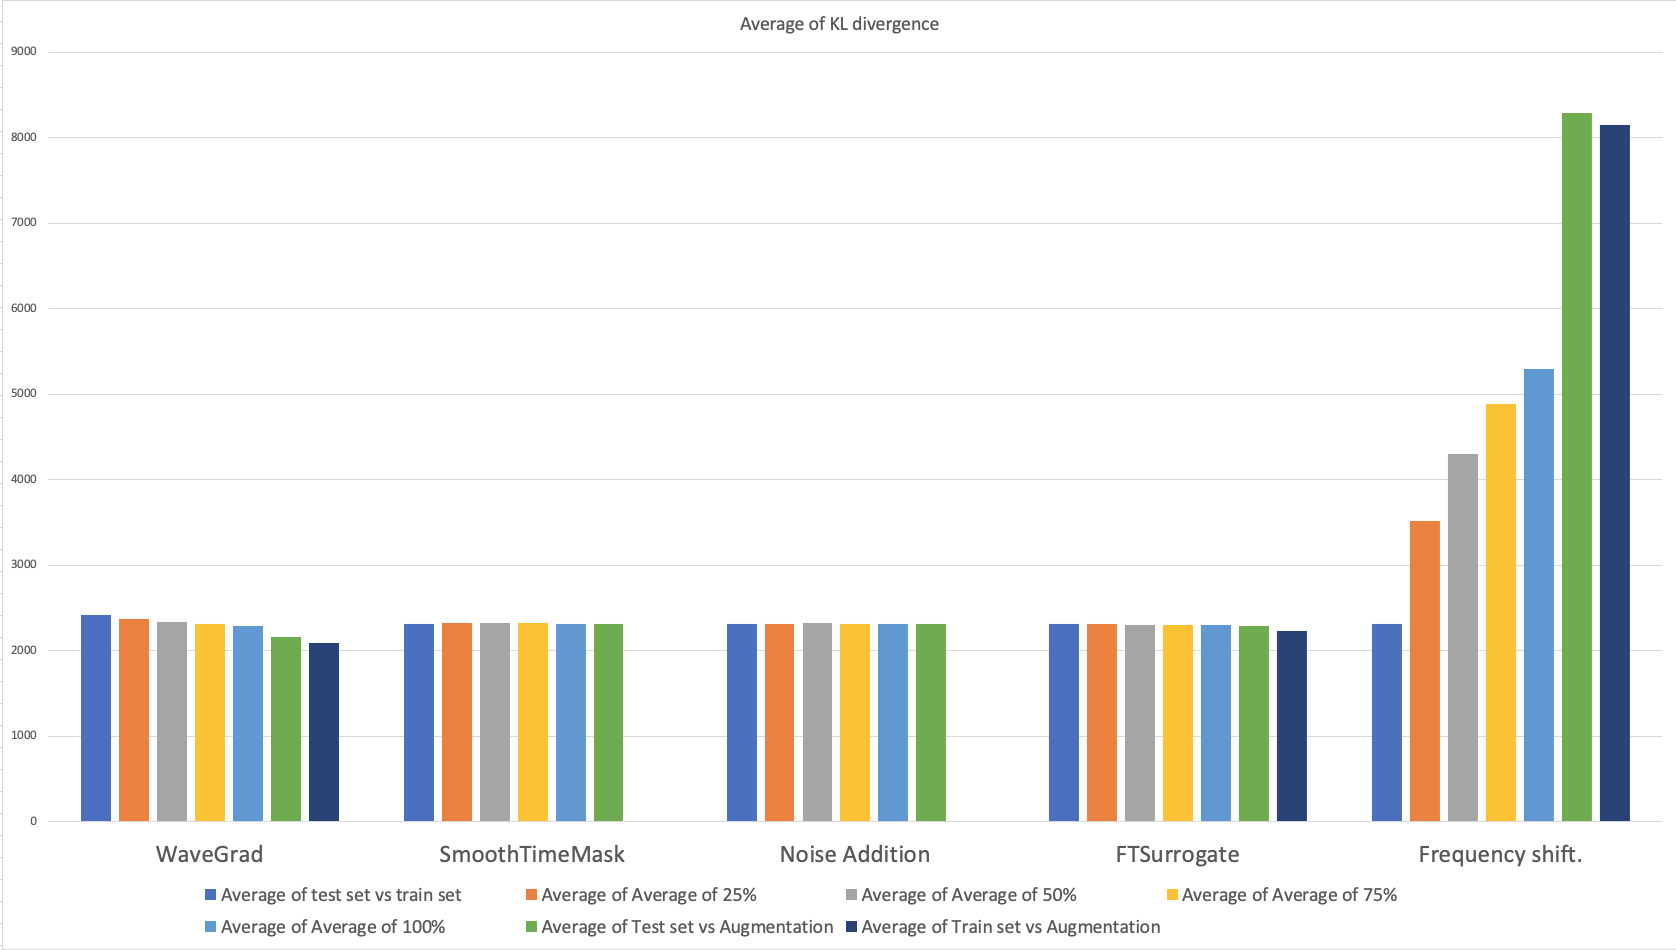
\includegraphics[width=1\textwidth]{fig/Avg_KL.png}
  \label{fig:Average of KL divergence}
\end{figure}


\subsection{Classification performance}
The baseline for the model was established by training it without any data augmentation, specifically without the use of synthetic data (i.e. 0\% synthetic data). The average accuracy of standard EEG MI classification models were presented on the Table \ref{table:Average accuracy of five standards EEG MI classification models}. 

Table \ref{table:Average accuracy of five standards EEG MI classification models} showed the average accuracy of five standard EEG motor imagery (MI) classification models using different data augmentation techniques. The baseline accuracy of the models was 42.45\%.  The results showed that the highest accuracy was achieved using the \texttt{WaveGrad} technique, with an accuracy of 51.15\%. This was an improvement of 8.7\% over the baseline accuracy. As shown in Table \ref{table:Average accuracy of five standards EEG MI classification models}, the highest accuracy values were obtained using \texttt{WaveGrad} (51.15\%) and \texttt{Frequency Shift} (43.07\%) techniques. The other two techniques, \texttt{Noise Addition} and Fourier transform surrogates, also improved the accuracy of the model to varying degrees. The \texttt{\texttt{SmoothTimeMask}} technique also resulted in higher accuracy values compared to the baseline, with the highest accuracy value of 38.84\% obtained at a 25\% size percentage.

%The results also show that as the size of the data augmentation increases, the accuracy of the models generally increases. For example, when using the \texttt{WaveGrad} technique, the accuracy increases from 50.56\% to 51.64\% to 50.78\% for 50\%, 75\%, and 100\% data augmentation, respectively. The table also includes the average accuracy of the five models using all the techniques, which is 51.03\%. The standard deviation of the average accuracy is 0.47\%. Overall, the results demonstrate that using data augmentation techniques can significantly improve the accuracy of standard EEG MI classification models.

Overall, our results demonstrated that DA techniques can be effective in improving the accuracy of EEG MI classification models. \texttt{WaveGrad} and \texttt{Frequency Shift} techniques were particularly promising, and were worth further investigation for future studies. Additionally, the size percentage of the DA techniques appeared to have an impact on model performance, suggesting that careful consideration of the amount of DA used was important for optimizing model accuracy. 

\begin{table}[ht] 
\centering
\caption{\label{table:Average accuracy of five standards EEG MI classification models} Average accuracy of five standards EEG MI classification models}
\scalebox{0.5}{
\begin{tabular}{|ll|ll|ll|ll|ll|ll|}
\hline
Baseline Accuracy(\%) & Size DA & \texttt{WaveGrad} (\%) & $\sigma$ & \texttt{Noise Addition}(\%) & $\sigma$ & \texttt{Frequency Shift}(\%) & $\sigma$ & Fourier transform surrogates(\%) & $\sigma$ & SmoothTimeMas(\%) & $\sigma$ \\ \hline
\textbf{42.45} & 25\% & \textbf{51.15} & 17.61 & 35.83 & 13.95 & \textbf{43.07} & 18.28 & 41.25 & 14.31 & \textbf{38.84} & 12.38 \\
& 50\% & \textbf{50.56} & 17.38 & 33.46 & 11.10 & 44.49 & 17.82 & 37.03 & 10.85 & 36.27 & 10.84 \\
& 75\% & 51.64 & 17.24 & 33.77 & 11.23 & 43.58 & 18.25 & 37.01 & 10.14 & 34.95 & 10.73 \\
& 100\% & 50.78 & 17.72 & 31.39 & 8.84 & 42.61 & 18.80 & 36.20 & 11.03 & 34.31 & 9.51 \\ \hline
\multicolumn{2}{l|}{Average Accuracy (\%)} & 51.03 & 17.49 & 33.86 & 11.53 & 43.44 & 18.04 & 37.12 & 11.08 & 36.09 & 10.86 \\ \hline
\end{tabular}

}
\end{table}

\subsection{Size of augmentation}
We present the impact of data augmentation on the similarity by KL-divergence in Figure 3 \ref{fig:Average of KL divergence}. This result show that \texttt{WaveGrad} are improve similarity when incurred number of ratio of data augmentation to raw signal.
We present the impact on accuracy of ratio of data augmentation to raw signal  in Table 6 \ref{table:Average accuracy of five standards EEG MI classification models}. This result show that the \texttt{WaveGrad} are not improve the accuracy.




\section{Discussion}
In this study, we demonstrated the implementation of the \texttt{WaveGrad}-based Diffusion Model as a DA for EEG MI datasets. From the result, our method performed the accuracy based on the standard EEG MI classification models more than traditional DA. Thus, for the discussion section, we focused mainly on our method.

\subsection{Key improvement}

The proposed methodology increased the variety of training sets, leading to an enhancement in the quality of the training set. As shown in Figure \ref{fig:Average of KL divergence}, Our research indicated that our method enhanced the similarity of training sets with test set. The traditional DA (\texttt{Noise Addition}, \texttt{FTSurrogate}, and \texttt{SmoothTimeMask}) and training set without DA were the KL divergence are the most the same. 
Our method are improve the similarity of test set and train \ref{fig:Average of KL divergence} our method more over another method are not improve the similarity. Spacial on \texttt{smooth time mask} and \texttt{noise add} the augmentation are not different the train set moreover the Frequency shift augment the seem make the train set and test set are more defence when decreased  the similarity of train set and test set.


\subsection{Subjects level}

In terms of research findings, it was observed that the data augmentation accuracy was highest for subjects who exhibited the greatest accuracy according to the standard EEG MI classification models prior to the implementation of data augmentation techniques. Subject 3's baseline accuracy was recorded to be 56.95\% during the initial assessment. The research findings indicated that the accuracy for subject number 3 was improved by 15.46\% using the implemented method. In contrast, the DA method employed in our study exhibited low efficacy when applied to the subject, as indicated by the subpar accuracy observed in relation to established EEG MI classification models. 
Subject 5's baseline accuracy was measured to be 28.08\% in the study. The research findings indicate that a method has been implemented to enhance the accuracy of subject number 5, resulting in a 4.13\% improvement. Table \ref{table: The Average accuracy improvement from our method on subject level} displayed the mean increased in accuracy resulting from the implementation of our method.
 
%the subjects that accuracy based on the standard EEG MI classification models with out the DA more than 40\% our method are improve the accuracy more than 10\%. the accuracy changing are present in table \ref{table: The accuracy changing}.

\begin{table}[ht] 
\centering
\caption{\label{table: The Average accuracy improvement from our method on subject level} The Average accuracy improvement from our method on subject level}
\scalebox{1}{
\begin{tabular}{|l|l|l|}
\hline
Subjects & Baseline Accuracy & \begin{math} \Delta \end{math} of \texttt{WaveGrad} \\\hline
1        & 43.06             & 17.01             \\
2        & 29.24             & 6.46              \\
\textbf{3}        & \textbf{56.95}            & \textbf{15.36}             \\
4        & 37.08             & 7.77              \\
\textbf{5}        & \textbf{27.08}             & \textbf{4.13}              \\
6        & 29.58             & 4.01              \\
7        & 40.07             & 11.77             \\
8        & 53.19             & 8.18              \\
9        & 65.76             & 2.59              \\\hline
\end{tabular}
}
\end{table}





 %Three and nine are the subjects with the highest accuracy based on the standard EEG MI classification models. Their accuracy are show in table \ref{table: Success subjects Accuracy}. In table\ref{table:Subject-dependent accuracy improvement},  the accuracy improvement of subjects three and nine is shown. The \texttt{WaveGrad} is success on DA for subjects, those have height accuracy on one of the standard EEG MI classification models trained by training sets without DA. The subjects with the lowest accuracy based on the standard EEG MI classification models are numbers two and five. Their accuracy are show in table \ref{table: Unsuccessful subjects Accuracy}. In table\ref{table: Unsuccessful Subjects Accuracy Change}, the accuracy change of subjects two and five is shown. \texttt{WaveGrad} is unsuccessful on DA for subjects with poor accuracy on one of the standard EEG MI classification models trained with training sets without DA.

\subsection{Size of DA}
%The BCI competition IV dataset record training set and testing set defferlent day. 
 The relationship between the size of DA and the performance of standard EEG classification was not a direct variation. Table \ref{table: The Average accuracy improvement from our method} presented the average accuracy improvement achieved by our method on the DA size level. The limitations of the dataset that used to train the \texttt{WaveGrad} method have impacted its capacity to produce signals with greater valence. The observed limitation might account for the non-linear relationship between the size of the data augmentation and the corresponding increased in accuracy. Research suggested that increasing the number of samples may not necessarily lead to a significant enhancement in accuracy, particularly if the additional samples fail to encompass the complete spectrum of potential signal fluctuations.


However, despite this limitation, the \texttt{WaveGrad} method still outperformed the baseline accuracy on all levels of data augmentation, with the highest improvement achieved at a DA size of 75\%. This finding suggested that even with a limited dataset, data augmentation techniques such as \texttt{WaveGrad} can still be effective in improving the accuracy of motor imagery classification using EEG signals.

It was worth noting that the results presented in the table were based on a single dataset, and the effectiveness of the \texttt{WaveGrad} method varies with other datasets or signal processing tasks. Future studies should investigate the generalizability of the \texttt{WaveGrad} method and explore its potential for improving accuracy in other EEG-based classification tasks.

The study concluded that although the \texttt{WaveGrad} method's capacity to produce signals with higher valence is affected by the restricted dataset used for its training, the outcomes presented in the table indicated that the method can enhance the precision of the motor imagery classification task using EEG signals. Additional investigation was required to establish the applicability of the \texttt{WaveGrad} approach to alternative datasets and signal processing assignments.


 
 %From key succress, size of DA are not improve viriouse of training seu until colse grp of training set and test sets.

%The sizing of DA improve highest performance is 75\% of size of raw EEG MI dataset. From table \ref{table: The Average accuracy improvement from our method on DA size level}. This size DA highest improve accuracy that is 9.19\%. Moreover this size DA is robustest with lowest \begin{math} \sigma \end{math} is 17.24. However, 

\begin{table}[ht] 
\centering
\caption{\label{table: The Average accuracy improvement from our method on DA size level} The Average accuracy improvement from our method on DA size level}
\scalebox{1}{
\begin{tabular}{|l|l|l|l|l|}\hline
Baseline Accuracy & DA size & \texttt{WaveGrad} & \begin{math} \sigma \end{math} & \begin{math} \Delta \end{math} \\ \hline
42.45             & 25\%    & 51.15    & 17.61                        & 8.71              \\
                  & 50\%    & 50.56    & 17.38                        & 8.11              \\
                  & 75\%    & 51.64    & 17.24                        & 9.19              \\
                  & 100\%   & 50.78    & 17.72                        & 8.33              \\ \hline
\end{tabular}
}
\end{table}


%\subsection{Standard EEG MI classification models performance}
%EEG signal have gap of distribution between each time of recording.
%Out method highest improve the performance on the standard EEG MI classification model that not complicate model bacaus
%The size of DA DA เพิ่มความหลากหลายแต่ DA miss gap of distribution between each time of recording but not at all then when add more did not improve the virious of training set.  Then %compicate model are rsik to over fiitign on training set and can not miss grp beween training set and test set.

\begin{table}[ht] 
\centering
\caption{ The Average accuracy improvement from our method.}\label{table: The Average accuracy improvement from our method}
\scalebox{1}{
\begin{tabular}{|l|l|l|l|l|} \hline
Model           & Baseline Accuracy & \texttt{WaveGrad} & \begin{math} \sigma \end{math} & \begin{math} \Delta \end{math} \\ \hline
ATCNet          & 47.68             & 53.63    & 18.45                        & 5.94  \\
Deep ConvNet    & 32.60             & 52.93    & 18.49                        & 20.33 \\
EEGITNet        & 46.84             & 54.96    & 16.76                        & 8.12  \\
EEGNet          & 34.18             & 37.04    & 8.00                         & 2.85  \\
ShallowFBCSPNet & 50.93             & 56.62    & 15.85                        & 5.69 \\ \hline
\end{tabular}
}
\end{table}

\subsection{Complexity of model}

The low complexity model our method are improve acculency more than hight complexity model because the hight complexity model are ez to overfitting on trainset. ref table 9  however our method are not decreed the accuracy.   \textcolor{red}{this paragraph looks off?}


\subsection{Limitation}
First, the proposed data augmentation method was developed based on a limited dataset, specifically the BCI competition IV dataset 2a. While the method showed promising results on this dataset, its effectiveness might be limited by the size and quality of the dataset used for its development. Future work could involve evaluating the generalizability of the method on other EEG MI datasets to improve its confidence in wider usage scenarios.  Second, the proposed data augmentation method was developed specifically for the EEG MI task. It might not necessarily generalize well to other EEG-based tasks. Future work could involve evaluating the method on other EEG signal tasks, such as P300 and SSEVP, to assess its robustness and adaptability across different EEG-based applications.

\section{Conclusion}
In this study, we investigated the effectiveness of data augmentation techniques on improving the accuracy of standard EEG MI classification models. We used five standard EEG MI classification models to classify EEG signals into left and right hand movements. We evaluated the performance of data augmentation techniques by comparing them with the baseline model, which were trained without any data augmentation. The data augmentation techniques, we used \texttt{WaveGrad}, \texttt{Noise Addition}, \texttt{Frequency Shift}, Fourier transform surrogates, and SmoothTimeMas.

Our results showed that data augmentation techniques improved the performance of standard EEG MI classification models, with \texttt{WaveGrad} being the most effective technique. The accuracy of the baseline model was 42.45\%, while the accuracy of the model trained with 75\% synthetic data generated by \texttt{WaveGrad} was 51.64\%. The other data augmentation techniques also improved the performance of the models, with \texttt{Noise Addition} and \texttt{Frequency Shift} being the least effective techniques.


\section{References}

% \bibliographystyle{iopart-num}
% \bibliographystyle{dcu}
\bibliographystyle{vancouver}
\bibliography{references}

\end{document}
